\section{Multistage Model}
%\subsection{Overview}

\begin{frame}{Multistage Model}
  \begin{itemize}
  \item stochastic dynamic equilibrium model
  \item long-run economic effects of strategic investment decisions
  \item oligopolistic market structure
  \end{itemize}
  \begin{itemize}
  \item multi-stage stochastic program with recourse
  \item uncertainty is reflected in future level of demand and strategic investment decisions 
  \item solution as mixed complementarity problem (MCP) with GAMS and PATH solver
   \item $S$-adapted open-loop information structure leads to Nash equilibria in each node 
  \end{itemize}
\end{frame}



%\subsection{Scenario Tree}

\begin{frame}{Scenario Tree}
\begin{center}
\psscalebox{0.60}{
\psset{nodesep=0pt,labelsep=1pt,nrot=:U}
\psmatrix[colsep=3.0cm,rowsep=0.0cm] 
                               &                                    &                                       & \circlenode{H}{$n_7$}\\ 
                               &                                    & \circlenode{D}{$n_3$}\\  
                               &                                    &                                       & \circlenode{I}{$n_8$}\\              
                               &  \circlenode{B}{$n_1$} & & \\
                               &                                    &                                       & \circlenode{J}{$n_9$}\\ 
                               &                                    & \circlenode{E}{$n_4$}\\  
                               &                                    &                                       & \circlenode{K}{$n_{10}$}\\ 
    \circlenode{A}{$n_0$} &                          &              & \\
                               &                                    &                                       & \circlenode{L}{$n_{11}$}\\ 
                               &                                    & \circlenode{F}{$n_5$}\\  
                               &                                    &                                       & \circlenode{M}{$n_{12}$}\\              
                               &  \circlenode{C}{$n_2$} & & \\
                               &                                    &                                       & \circlenode{N}{$n_{13}$}\\ 
                               &                                    & \circlenode{G}{$n_6$}\\  
                               &                                    &                                       & \circlenode{O}{$n_{14}$}\\ 
& & & \\
 $t=0$ & $t = 1$ & $t=2$ &  $t=3$\\
\ncline[linewidth=1.5pt]{A}{B}\naput{$50\%$}
\ncline[linewidth=1.5pt]{A}{C}\naput{$50\%$}
\ncline[linewidth=1.5pt]{B}{D}\naput{$25\%$}
\ncline[linewidth=1.5pt]{B}{E}\naput{$25\%$}
\ncline[linewidth=1.5pt]{C}{F}\naput{$25\%$}
\ncline[linewidth=1.5pt]{C}{G}\naput{$25\%$}
\ncline[linewidth=1.5pt]{D}{H}\naput{$12.5\%$}
\ncline[linewidth=1.5pt]{D}{I}\naput{$12.5\%$}
\ncline[linewidth=1.5pt]{E}{J}\naput{$12.5\%$}
\ncline[linewidth=1.5pt]{E}{K}\naput{$12.5\%$}
\ncline[linewidth=1.5pt]{F}{L}\naput{$12.5\%$}
\ncline[linewidth=1.5pt]{F}{M}\naput{$12.5\%$}
\ncline[linewidth=1.5pt]{G}{N}\naput{$12.5\%$}
\ncline[linewidth=1.5pt]{G}{O}\naput{$12.5\%$}
\endpsmatrix}
\end{center}
\end{frame}

\begin{frame}{Notation}
  \begin{tabular}[l]{l l}
\centering
$i \in \mathcal{I}$ & players, firms \\
$j \in \mathcal{J}$ & available technologies \\
$m\in\mathcal{M}$ & market states \\
$p_n$ & probability to reach a certain node\\
$p^m$ & probability of market state $m$ \\
$ q_{i,n}^{j,m}$ & production quantities \\
$I_{i,n}^{j}$ & investment quantities, for $n\in\left\{n_0\right\}\cup\mathcal{T}$ \\
$K_{i,n}^{j}$ & available capacity\\
$F_n^{j}$ & investment cost\\
$P^m_n = \alpha_n^m-\beta^m\sum_{i\in \mathcal{I}}\sum_{j\in \mathcal{J}}q_{i,n}^{j,m}$ & market equilibrium price \\
$\alpha_n^m$ & intercept of demand function \\
$\beta^m$ & slope of demand function \\
$c_j$ & variable costs \\
$\delta_n$ & discount factor \\
$\nu$ & salvage value parameter\\
$\rho$ & depreciation rate\\
\end{tabular}
\end{frame}

\begin{frame}{Optimization}

\begin{equation}
  \label{eq:objfct}
  \max_{q_{i,n}^{j,m}, I_{i,n}^{j}} \sum_{n\in \mathcal{N}}p_n\delta_n\Pi_{i,n}\left(q_{i,n}^{j,m}, I_{i,n}^{j}, K_{i,n}^{j}, Q_n^m\right)+ \sum_{n\in \mathcal{S}}p_n\,\delta_n \sum_{j\in \mathcal{J}}K_{i,n}^{j}F_n^{j}\nu
\end{equation}
subject to
  
\begin{eqnarray}  
q_{i,n}^{j,m} - K_{i,n}^{j} &\leq& 0 \quad \forall i,j,m,n \label{eq:prodconstr} \\
Q_n^m-\sum_{i\in \mathcal{I}}\sum_{j\in \mathcal{J}} q_{i,n}^{j,m} &=& 0 \quad \forall m,n \label{eq:marketclearing}\\
K_{i,n}^{j} - (1-\rho)K_{i,a(n)}^{j}-I_{i,a(n)}^{j} &=& 0 \quad \forall i,j,n \label{eq:state} \\
q_{i,n}^{j,m}, K_{i,n}^{j}, I_{i,n}^{j}, Q_n^m  &\geq& 0 \quad \forall i,j,m,n\label{eq:nonneg}
\end{eqnarray}
  
\end{frame}



\section{The German Electricity Market}

\subsection{Installed Capacities}

\begin{frame}{Installed Capacities}
					
\begin{figure}[h]
  \centering
%\caption{Installed capacities in GW of major players in Germany}
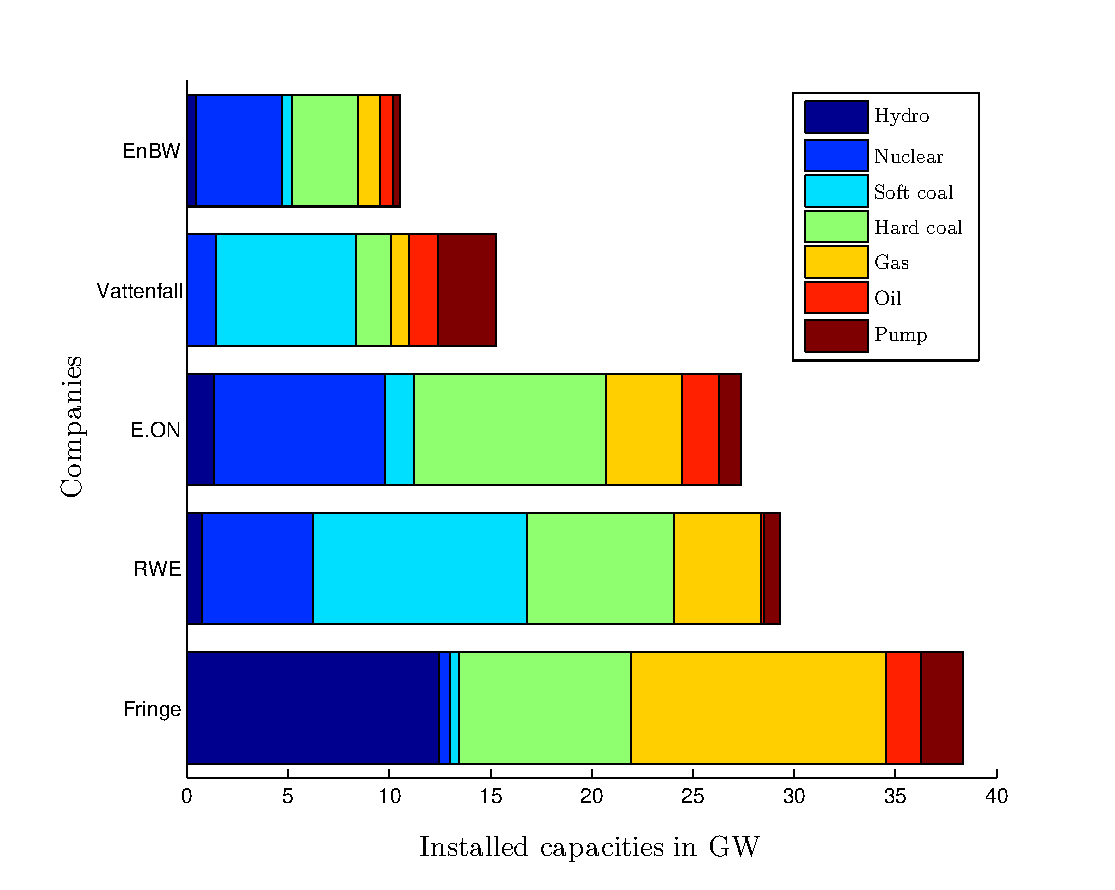
\includegraphics[width=0.8\textwidth]{capacities}
  \label{fig:capacities}
\\
\vspace{0.1cm}
\scriptsize Source: International Energy Agency (2007)
\end{figure}

\end{frame}

\subsection{Electricity Load and Prices}

\begin{frame} {Electricity Load}
					
\begin{figure}[h]
\centering
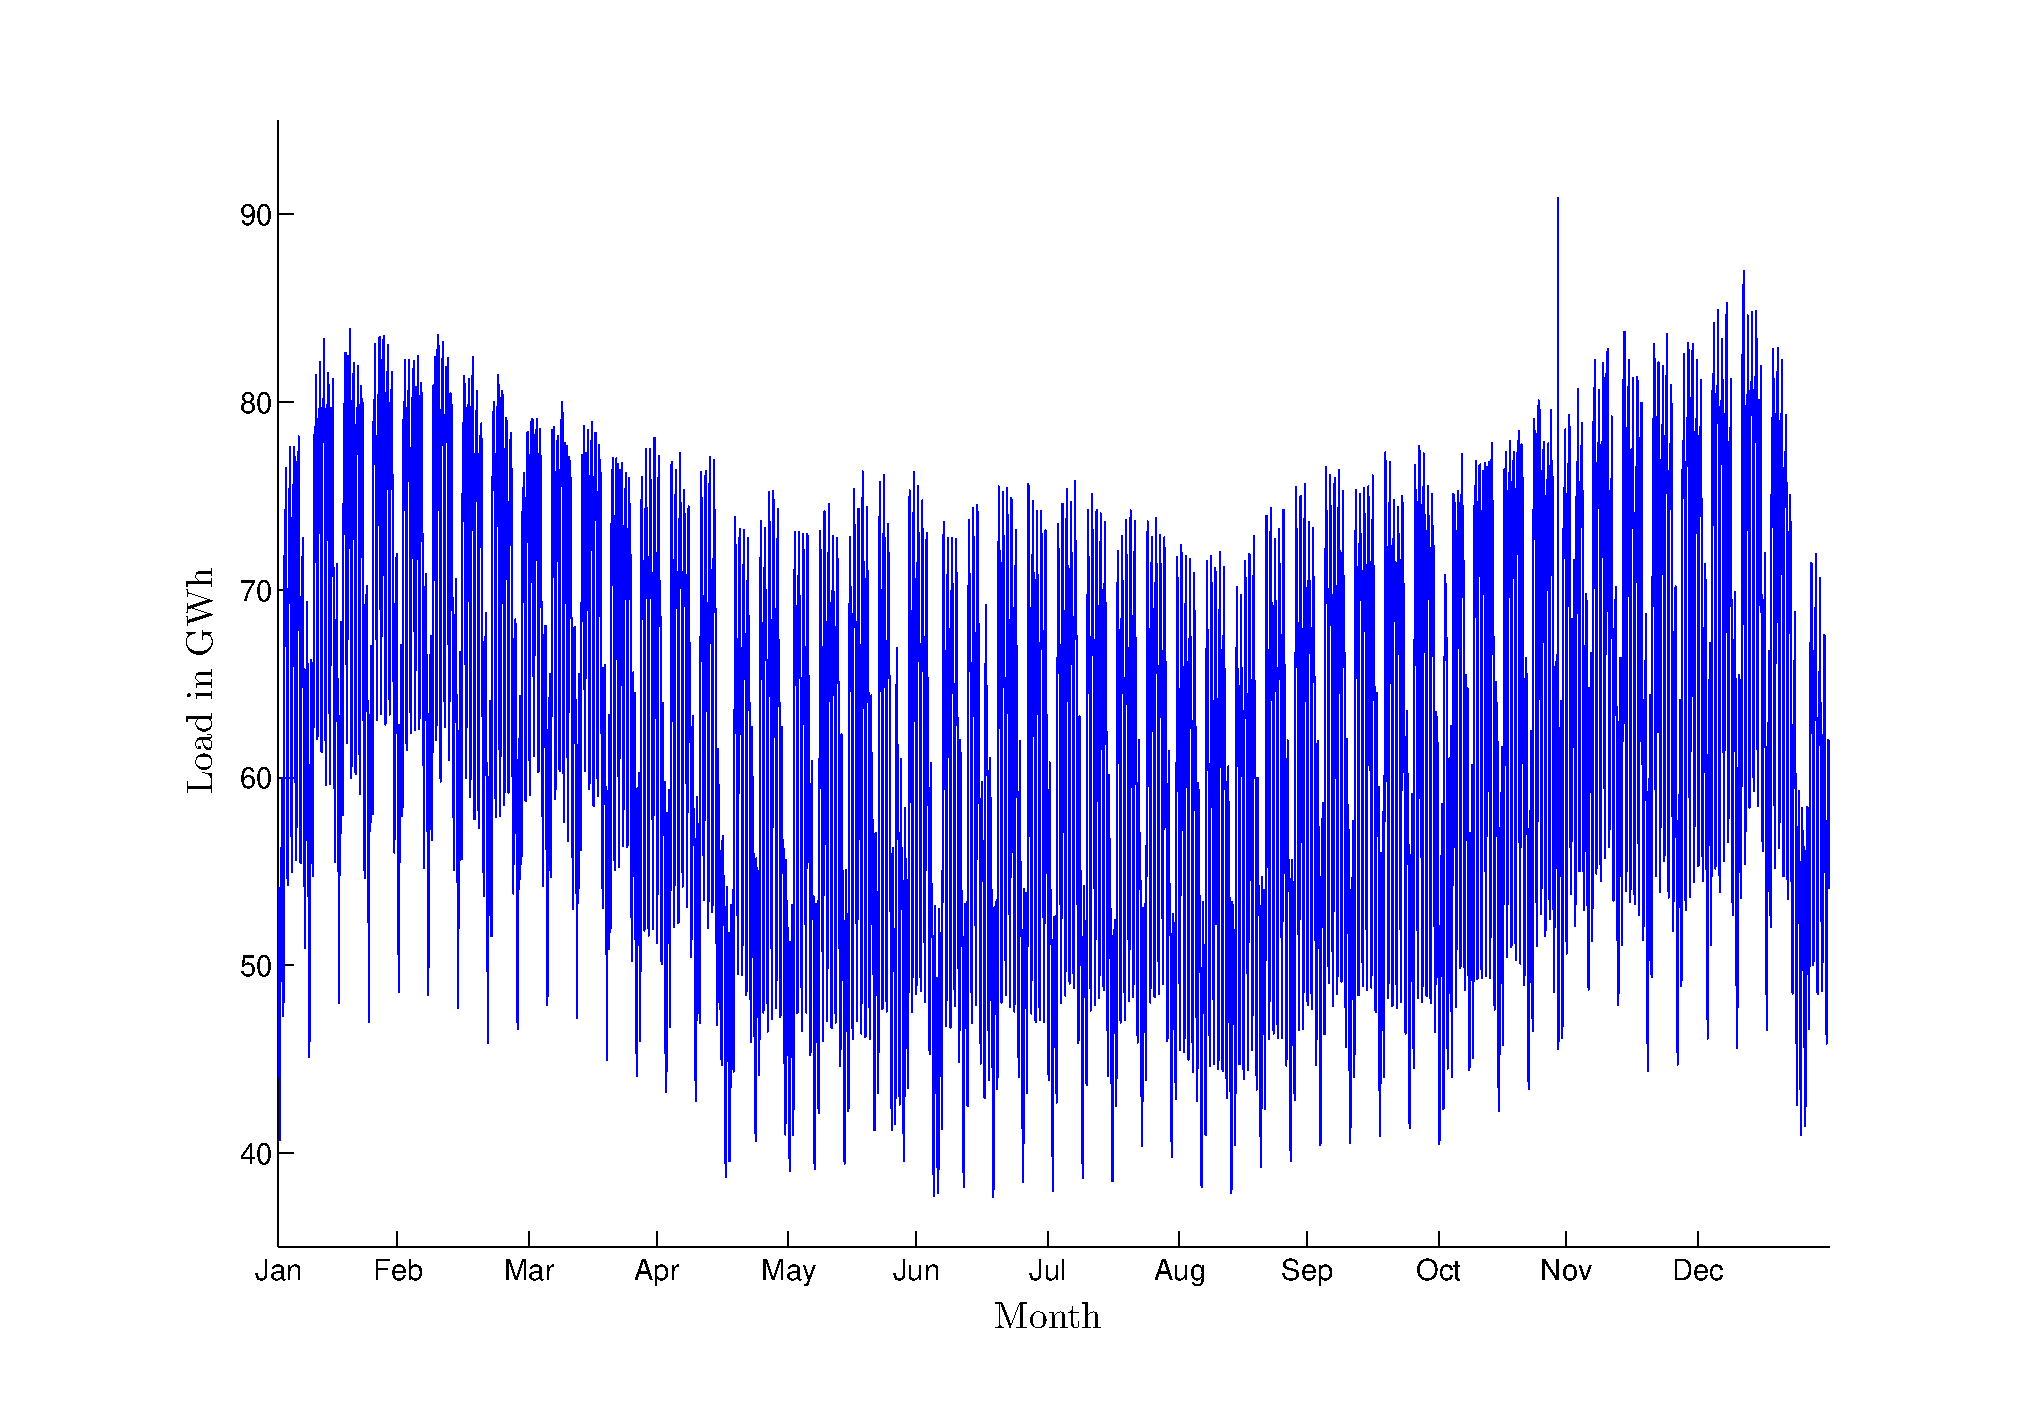
\includegraphics[width=0.9\textwidth, angle=0]{loadvalues}
    \label{fig:load}   
\\ 
\vspace{0.1cm}
\scriptsize Source: UCTE (2006)           
\end{figure}
\end{frame}

\begin{frame} {Electricity Prices}				
\begin{figure}[h]
\centering
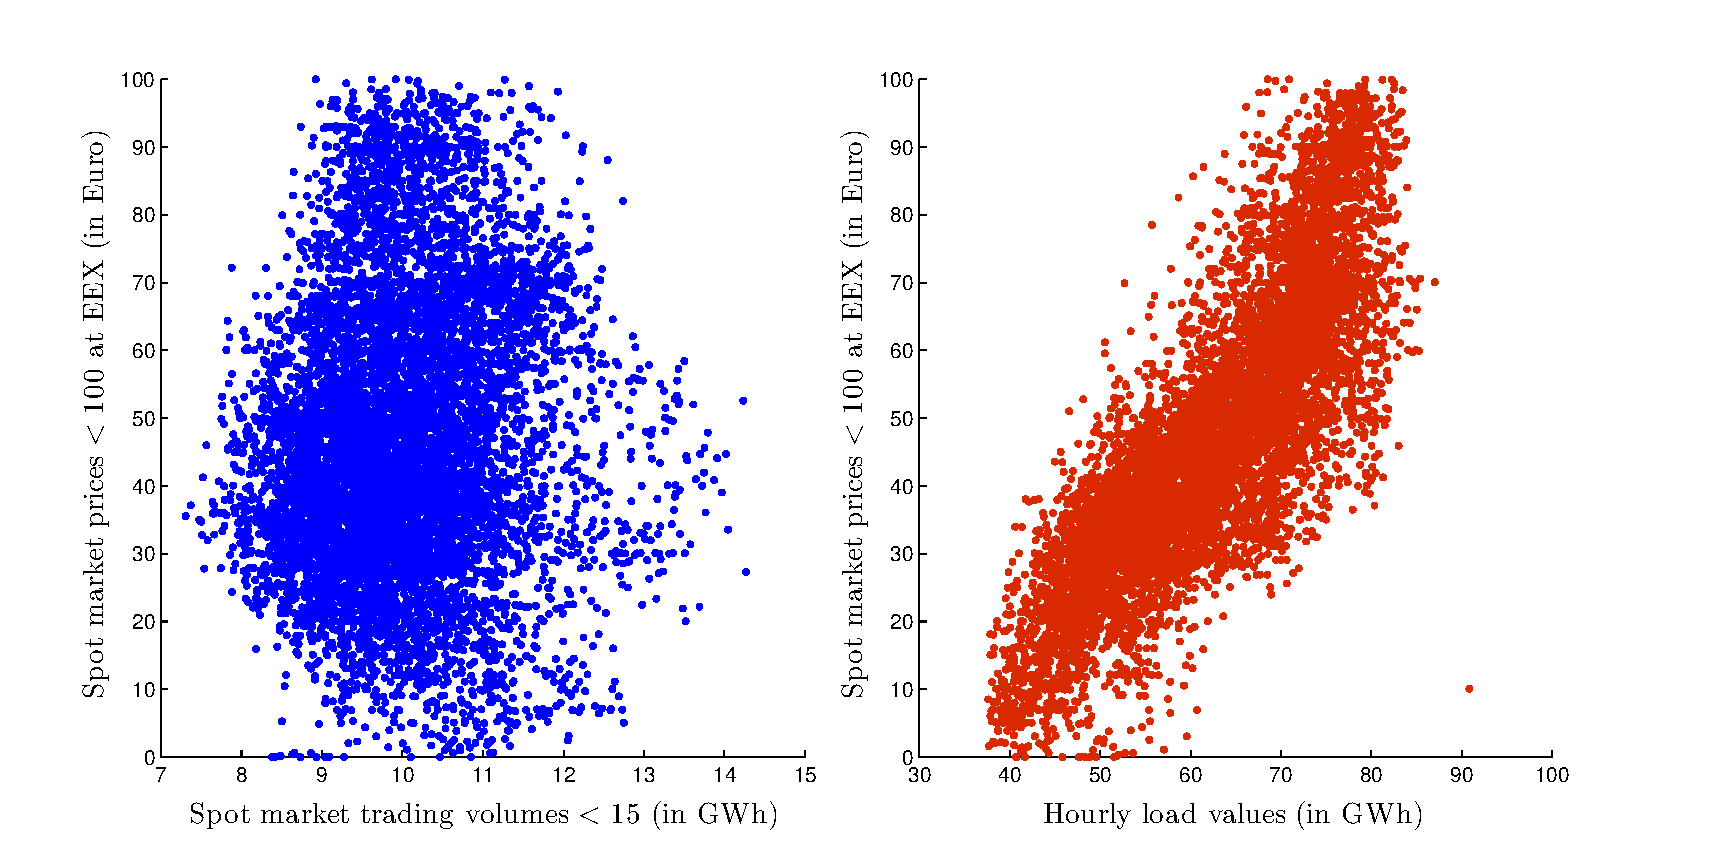
\includegraphics[width=1.0\textwidth, angle=0]{pricequant}
    \label{fig:load} 
\\ 
\vspace{0.1cm}
\scriptsize Source: EEX (2006); UCTE (2006)           
\end{figure}
\end{frame}

\begin{frame}
  \frametitle{Market Segments}

\begin{center}
\small
\begin{tabular}{rrrrr}
  \hline
Price & Average price  & Average quantity & Number of & Percentage of \\
intervals& (Euro/MWh) &  (MWh) &  prices & of total prices\\
  \hline\hline
$0\leq p<20$ & 12.67 & 46,111.63 & 611 & 6.98\% \\
$20\leq p<40$ & 31.35 & 54,103.50 & 3,003 & 34.28\% \\
$40\leq p<60$ & 49.00 & 64,806.04 & 2,626 & 29.98\% \\
$60\leq p<80$ & 68.46 & 72,385.56 & 1,588 & 18.13\% \\
$80\leq p<100$ & 88.40 & 75,991.21 & 665 & 7.59\% \\
$100\leq p<\infty$& 176.06 & 76,482.34 & 266 & 3.04\% \\
   \hline
\end{tabular}  
\normalsize
\end{center}

\end{frame}

\subsection{Marginal and Investment Costs}

\begin{frame}
  \frametitle{Marginal and Investment costs}
\begin{center}
  \begin{tabular}{rrr}
\hline
           & Variable costs & Investment costs\\
           &  (Euro/MWh)    &  (Euro/GW) \\
\hline\hline
     Hydro &        7.6 &    3,500\\

   Nuclear &        9.5 &    1,841 \\

   Lignite &       10.6 &    1,074 \\

 Hard coal &       16.1 &     971 \\

 Gas (CCGT) &       33.5 &     460 \\

Oil & 44            &   n/a\\

Pump &         80 &       n/a\\
\hline
\end{tabular}
\\
\vspace{0.3cm}
\scriptsize Source: Auer et al. (2006)
\end{center}
\end{frame}

\section{Results}

\subsection{Scenario Generation}

\begin{frame}
  \frametitle{Scenario Generation}
\begin{figure}[h]
  \centering
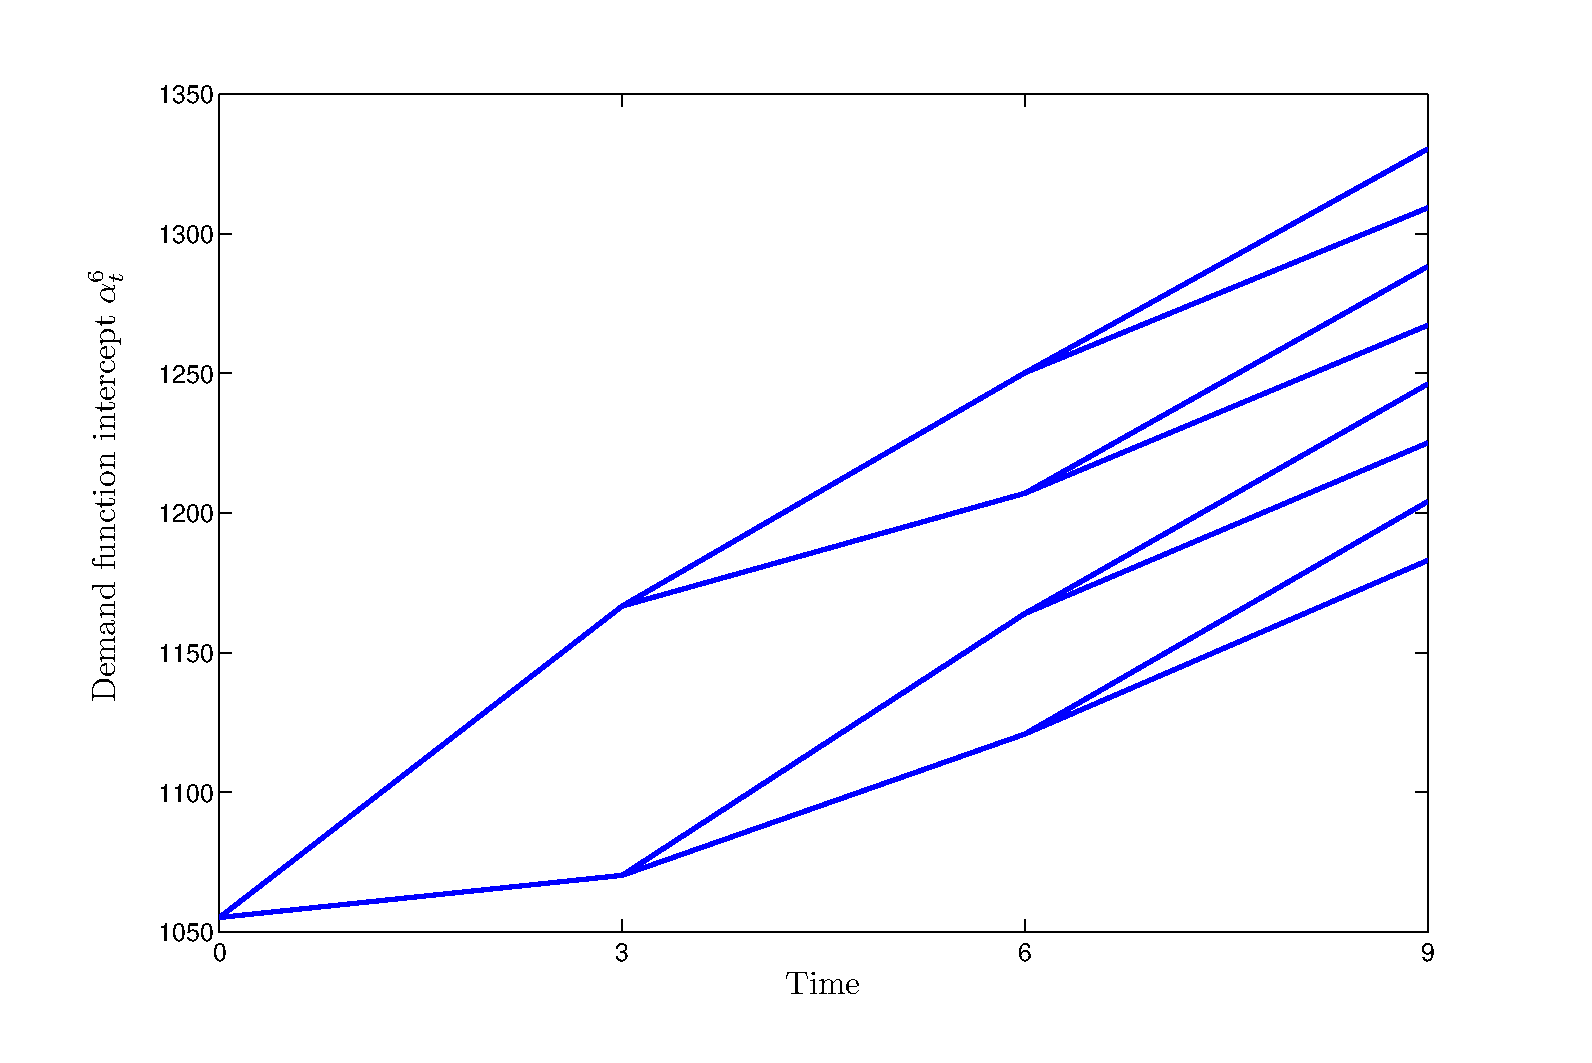
\includegraphics[width=1\textwidth]{intercept}
  \label{fig:intercept}
\end{figure}  
\end{frame}


\subsection{Solution of the MCP}

\begin{frame}
  \frametitle{Production in the initial node $q_{i,0}^{m}$ (in MWh)}
  \begin{center}
\scriptsize
      \begin{tabular}{rrrrrrr}
\hline
           &     $m=1$ &     $m=2$ &     $m=3$ &     $m=4$ &     $m=5$ &     $m=6$ \\
\hline\hline
       Rwe &    10,945.21  &    13,590.03  &    17,150.64  &    20,586.19  &    21,872.07  &    21,984.52  \\

       EON &    10,945.21  &    13,592.14  &    17,150.64  &    20,586.09  &    21,871.99  &    21,984.48  \\

    Vattenfall &    10,940.85  &    13,590.03  &    15,273.00  &    15,273.00  &    15,273.00  &    15,273.00  \\

      EnBW &    10,528.00  &    10,528.00  &    10,528.00  &    10,528.00  &    10,528.00  &    10,528.00  \\
\hline
\end{tabular}
\normalsize
  \end{center}
\end{frame}



\begin{frame}
  \frametitle{Sensitivity Analysis}

  \begin{itemize}
  \item Investment quantities in the initial node $I_{i,0}$ (in MW) with $\rho=0.025$
  \end{itemize}

\begin{center}
  \begin{tabular}{rrrrr}
\hline
           &       $\nu=0.99$ &       $\nu=0.95$ &        $\nu=0.9$ &       $\nu=0.85$ \\
\hline\hline
 Vattenfall  &      5,015.93  &      4,832.23  &      4,626.18  &      4,516.54  \\

     EnBW  &      9,582.64  &      9,405.55  &      9,229.64  &      9,120.00  \\
\hline
\end{tabular}
\end{center}

\begin{itemize}
\item Investment quantities in the initial node $I_{i,0}$ (in MW) with $\nu=0.95$
\end{itemize}

\begin{center}
  \begin{tabular}{rrrrr}
\hline
           &      $\rho=0.025$ &       $\rho=0.03$ &      $\rho=0.035$ &       $\rho=0.04$ \\
\hline\hline
Vattenfall &      4,832.23  &      4,908.60  &      4,984.96  &      5,061.33  \\

      EnBW &      9,405.55  &      9,458.19  &      9,510.83  &      9,563.47  \\
\hline
\end{tabular}  
\end{center}

\end{frame}